\documentclass[english, a4paper, 12pt, twoside]{article}
\usepackage[margin=2.64cm]{geometry}
\usepackage{graphicx}
\usepackage{amsmath, amsfonts}
\usepackage{amssymb}
\usepackage{subcaption}
\linespread{1.25}
\usepackage{rotating} %sideways figure
\usepackage{pdflscape}
\usepackage{verbatim}

\usepackage[utf8x]{inputenc}
\usepackage[T1]{fontenc}

\usepackage{lmodern}
\usepackage{textcomp}
\usepackage{fancyhdr}

\usepackage[round]{natbib}
%\usepackage{biblatex}
%\addbibresource{references.bib}

% \usepackage{babel}

% \usepackage{titlesec}

\usepackage[font=footnotesize]{caption}

\usepackage{xcolor}

\usepackage{hyperref}

\usepackage{gensymb}
\hypersetup{
    colorlinks,
    linkcolor={red!50!black},
    citecolor={blue!50!black},
    urlcolor={blue!99!black}
}

\usepackage{titling}

% ----- Header and footer -----
\pagestyle{fancy}
\fancyhead[RO,LE]{\thepage} % page number on right for odd pages and left for even pages in the header
\fancyhead[RE,LO]{\nouppercase{\rightmark}} % chapter name and number on the right for even pages and left for odd pages in the header
%\renewcommand{\headrulewidth}{0pt} % sets thickness of header line
\fancyfoot{} % removes page number on bottom of page

% ----- Header of the frontpage ----- 
\fancypagestyle{frontpage}{
	\fancyhf{}
	\renewcommand{\headrulewidth}{0pt}
	\renewcommand{\footrulewidth}{0pt}
	\vspace*{1\baselineskip}
	
	\fancyhead[R]{UFR PhITEM
	\linebreak       Grenoble, spring 2019\vspace*{5\baselineskip}}
	\fancyhead[L]{ 
\includegraphics[width=1.4in]{fig/logo_UGA.png}}
}


% ----- Document starts here ----- 

\pretitle{%

\includegraphics[width=0.3\linewidth]{fig/logo_UGA}
\vspace{2cm}
\begin{center}
\LARGE
}
\posttitle{\end{center}
\vspace{1cm}
}
\postdate{\par\end{center}\vspace{12cm}~}

\usepackage[nottoc,numbib]{tocbibind}
\usepackage{footnote}
\makesavenoteenv{tabular}
\makesavenoteenv{table}
%%%%%%%%%%%%%%%%%%%%%%%%%%%%%%%%%%%%%%%%%%%%%%%%%%%%%%%%
%%%%%%%%%%%%%%%% COVER %%%%%%%%%%%%%%%%%%%%%

\begin{document}
\linespread{1.5}

\begin{titlepage}
	
	\newgeometry{top=1 in, bottom=1 in, left=1 in, right= 1 in} 
	
	\thispagestyle{frontpage}
	
	\begin{center}
		
		\vspace*{8\baselineskip}
	
		
		{\Huge \textbf{Measurements of Turbulence in Katabatic Wind on a steep slope\\}}
		
		
        \vspace*{1,5\baselineskip}

		\large{\textbf{Claudio Pierard}}\\
		\large{\textbf{Supervisor: Dr. Jean-Emannuel Sicart}}\\
		
		\vspace{1,5\baselineskip}
		
		\large{Master 1 Applied Mechanics}\\
		\large{Reasearch Project}\\
		
		\vspace{1,5\baselineskip}
		\large{UNIVERSITÉ GRENOBLE ALPES}\\

	\end{center}
	
\end{titlepage}
\restoregeometry % restores the margins after frontpage
%\nocite{*} % uncomment if you want all sources to be printed in the reference list, including the ones which are not cited in the text 

\pagenumbering{gobble} % suppress page numbering
\thispagestyle{plain} % suppress header
\clearpage\mbox{}\clearpage % add blank page

\pagenumbering{roman} % starting roman page numbering
\newpage
\linespread{1.25}
\section*{Abstract}
    [Must modify this abstract] The study of katabatic winds is relevant because it influences the weather and pollution condition of the valleys in mountainous regions. We propose a field case study of the katabatic winds in the Belledonne Massif, with the objective of measuring the turbulence of the downslope jet and characterise it. We present the basic concepts necessary to study the katabatic winds and the objectives for the proposed project based on previous studies done by students that worked on it before. In the end, a work plan or schedule is presented which describes the activities to do during the next months.

\newpage

\section*{Acknowledgements}
    Acknowledgements go here.
\newpage

\tableofcontents
\newpage
\listoffigures
%\listoftables

\newpage
\pagenumbering{arabic}

\section{Introduction}
Katabatic winds or gravity currents are downslope winds that are generated when cold dense air is accelerated down a topographic slope due to surface cooling that gives the air a greater density than the free atmosphere~\citep{poulos2008observational}. They can be found in many places over the world, but they are mostly present in cold mountainous regions and over glaciers. 

Katabatic winds play an important role in the local weather and the dispersion of contaminants in the valleys. These winds can flow down the mountains and fill the bottom of valleys with cooled air. This can result in a very cool layer of air that doesn't mix with the top layers, called temperature inversions, which have negative effects on urban valleys where pollution is present~\citep{largeron2016persistent}.

Nowadays, katabatic winds are not well parameterized in mesoscale models for weather forecast because the spatial scale at which this winds occur can't be represented with those models.... And is a potential source of errors in weather forecasts over mountainous regions. 

There are several studies of katabatic winds, mostly centred in the alpine regions of Europe, some parts of North America, Greenland and Antarctica, but despite this, there is a lack of suitable data obtained from measurements that can be used to test or adapt the theoretical models of katabatic winds~\citep{manins1979katabatic}(Too old). Most of these studies were performed on not very st

Alsleeop(not more than 10$\degree$)esp , which iparticular characteristic of the large Glaciers found in Antarctica and Greenland.s so, thea re are few studies of these winds on steep slopes, mostly these are focused in regions where the slopes is smaller than $10 \degree$.

In this section we introduce and define some of the concepts necessary for this project, starting from the boundary layer structure to the specifics of the turbulent quantities necessary for its characterisation.

\subsection{Boundary layer structure}
The planetary boundary layer or atmospheric boundary layer (ABL) is defined as the part of the troposphere that is in contact with the surface and that is directly influenced by surface forcings, such as friction, evaporation, heat transfer, emission of contaminants and by the soil~\citep{stull2012introduction}. The thickness or height of the ABL varies throughout the day and depends on the location. Mainly the height varies by the incidence of solar radiation on the surface, which makes the air parcels in contact with the surface acquire more flotation, generating convection.

\begin{figure}[ht!]
	\vspace{-5pt}
    \centering
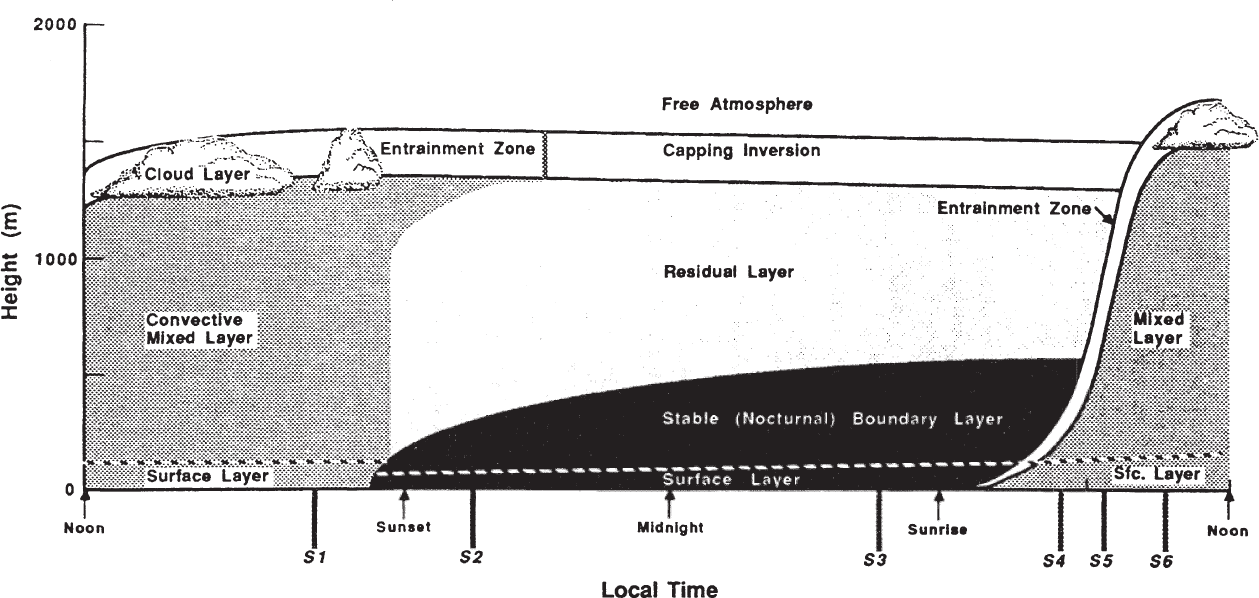
\includegraphics[width=0.9\textwidth]{fig/abl_stull.png}
    \caption{Diagram of the daily evolution of the structure of the ABL. Image based on \cite{stull2012introduction}.}
    \label{fig:ABL_structure}
  \vspace{-5pt}
\end{figure}

The figure~\ref{fig:ABL_structure} shows the structure and temporal evolution of the ABL, its components are the mixing layer, the residual layer and the stable boundary layer. Each of these has special characteristics and different physical processes that distinguish them. To understand the dynamics of the planetary boundary layer it is necessary to define each of them. However, in this study, we focus mostly on the stable nocturnal boundary layer because in the presence of this layer katabatic winds form~\citep{poulos2008observational, stull2012introduction}.

\subsubsection{Stable boundary layer}
The stable nocturnal boundary layer is formed during the night when the sunlight stops reaching the ground and therefore starts cooling down. This layer is characterised by sporadic turbulence caused by wind shear and the contact with the surface, which tends to suppress turbulence. The upper limit of the stable boundary layer is located at the height where the intensity of the turbulence is a small fraction of its surface value. The air in this layer is statically stable, opposed as its daytime equivalent, the mixed layer~\citep{stull2012introduction}.

When the stable boundary layer is formed, the air that is close to the ground cools down and can form drainage winds or katabatic winds, over a slope in the topography.

\subsection{Katabatic wind}

The katabatic winds are local winds that are created over a descending terrain gradient when air masses flow downslope, being cooled by radiative processes near the ground. These winds are a ventilation mechanism in mountainous regions~\citep{manins1979model}. Normally, these winds are shallow, where the thickness of the jet can go up to 2-3~m, with velocities on the order of 1 to 5~m/s \citep{stull2012introduction}. 

\begin{figure}[ht!]
	\vspace{-5pt}
    \centering
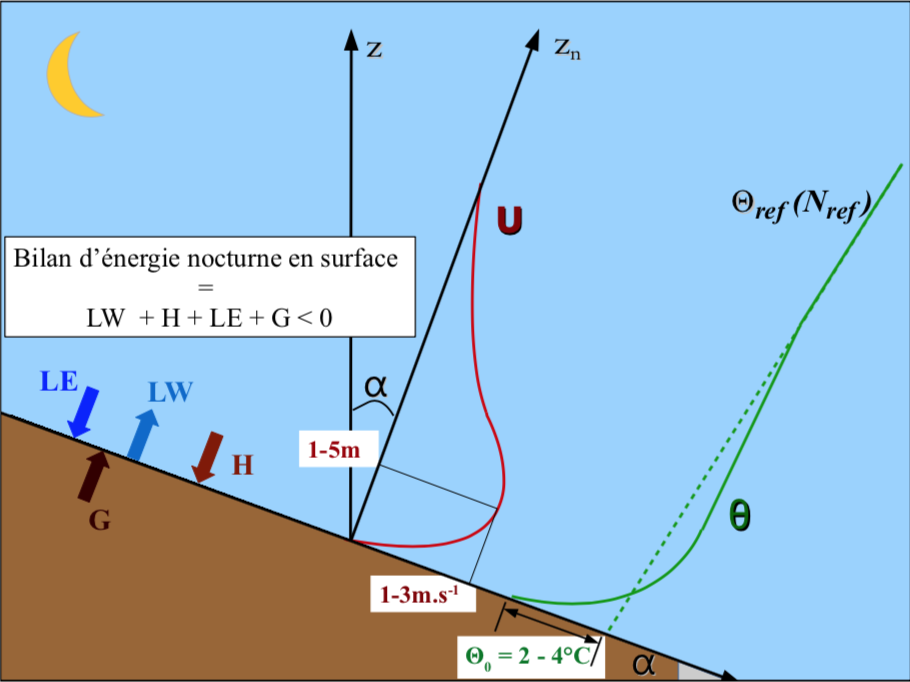
\includegraphics[width=0.6\textwidth]{fig/profiles_katabatic_wind.png}
    \caption{Characteristic wind profile (red) and potential profile (green) of the katabatic wind. Image from~\cite{claudine}.}
    \label{fig:u_profile}
  \vspace{-5pt}
\end{figure}

These winds are characterised for having a velocity profile as the one shown in the red curve in figure~\ref{fig:u_profile}. We can see that near the surface the velocity grows as we go up until it reaches a maximum and starts to decrease. The maximum is close to the surface. This is the theoretical velocity profile of the katabatic winds. Also in figure~\ref{fig:u_profile}, we can see in the green curve the profile for the potential temperature, where we the theoretical profile shows that it grows rapidly as we go up until a point were it remains constant. This theoretical results can be useful to detect the occurrence of katabatic wind in the data sets.

An important factor to highlight about the katabatic winds is that external factors like synoptic or mesoscale winds can alter or destroy this kind of local winds~\citep{stull2012introduction}. The katabatic winds are important under conditions of slack synoptic pressure gradients~\citep{manins1979katabatic}. This factor plays an important role in the planning out the field campaign because we want to measure the katabatic jet as undisturbed as possible. For this, we are looking for a meteorological window when anticyclonic conditions will be present. 

\subsection{Turbulence Kinetic Energy (TKE)}
The TKE is defined as the kinetic energy per unit mass. This is one of the most important quantities to characterise turbulence in a flow, by giving us information about whether a region will become more turbulent, or whether turbulence will decay~\citep{stull2012introduction}.  Is defined as:

\begin{equation}
    e = \frac{1}{2} \big(\overline{u'^2} + \overline{v'^2} + \overline{w'^2}\big). 
    \label{eq:tke}
\end{equation}

\noindent where $e$ is the definition of turbulent kinetic energy (TKE). Is the sum of the variances of the wind components fluctuation. The over-line represents the average of the variable. 

\subsection{Covariance}

Recalling the classical definition of covariance between to variables, we have the relation 

\begin{equation}
    \text{covar}(A,B) = \frac{1}{N}\sum_{i=0}^{N-1} (A_i - \overline{A})(B_i - \overline{B}).
\end{equation}

\noindent Using the Reynolds averaging method in the previous expression we get:

\begin{subequations}
\begin{align}
    \text{covar}(A,B) &= \frac{1}{N}\sum_{i=0}^{N-1} a_i' b_i', \\
    &= \overline{a'b'}.
\end{align}
\end{subequations}

\noindent This is the mathematical definition of covariance. The covariance indicates the degree of common relationship between two variables. Is the principle by which we define the eddy fluxes.

\subsection{Eddy Flux}
According to \cite{stull2012introduction}, a turbulent flux or eddy flux is the transport of a physical quantity by the effect of the turbulence. In this project, we are mostly concerned with the sensible heat flux and the momentum flux. The sensible heat flux is given by the expression:

\begin{equation}
    H = \rho \ C_p \ \overline{w'\theta'},
\end{equation}

\noindent where $C_p$ is the specific heat at constant pressure and $\theta '$ is the fluctuations in potential temperature. We are interested in the vertical flux of the sensible heat, that is why we use the vertical wind fluctuation $w'$.

The momentum flux is given by the expression

\begin{equation}
    F = \rho \ \overline{u'w'}, 
\end{equation}

\noindent where $\rho$ is the density of air, and $u'$ and $w'$ are the fluctuations of velocity in the x-coordinate and in the vertical coordinate. The x-coordinate follows the slope and the z-coordinate is perpendicular to the slope. The latter expression also is known as a component of the \textbf{Reynolds stress tensor}. The Reynolds stress describes all the components of the momentum flux in a control volume.


\section{Theory}
%My project is based on the work done by previous students, who made their master thesis on the same subject but with different data sets obtained from previous field campaigns. In Particular, \cite{jakob} processed the data of the 2015 campaign, that took place from 7 to 22 April 2015, during an episode of anticyclonic conditions. In his work, he had to detect the days in which the instruments measured katabatic winds. For this, he used the past records of the meteorological report to see when there were anticyclonic weather conditions. Also, he analysed the wind profiles and temperature profiles to see if they fitted the description of the katabatic winds. After selecting the days, he computed the Reynolds stress tensor, the sensible heat flux and the turbulent kinetic energy. Is important to highlight that he analysed the region where the maximum of the velocity of the jet is expected to be. As a suggestion for future projects, he points out that it could be interesting to study the turbulence beneath the wind maximum, by placing more sensors in the lower levels of the masts (see section~\ref{instrumentation}).

%Also, my work takes in to account the previous work done by \cite{claudine} and \cite{alban}. Both of them analysed the data from the November 2012 campaign. They followed the same methodology as \citeauthor{jakob} did, analysing the same turbulence characteristics of the jet. The main difference is that their work is focused on adapting the Prandtl analytical model with the different measurements recorded in the field. Another difference is that \citeauthor{claudine} did a spectral analysis of the data. This allowed her to represent the energy as a function of the frequency, with the objective to see the energy cascade characteristic of turbulence. 

\subsection{Objectives}
My objectives for this research project will be to analyse the data from a new mission planned for this the months of January or February, in which there are more sensors installed especially in the bottom and the lower region of the meteorological stations (see section~\ref{instrumentation}). This tackles the limitations found in the previous works mentioned above. 

More specifically, the first step will be to pre-process the data using the EddyPro Software (eddy covariance method). Then, it will be necessary to detect the katabatic wind episodes in the data set, by selecting the data that coincide with the anticyclonic episodes and which temperature and wind profiles coincide with the description of the katabatic winds. After that, I will analyse all the turbulent characteristics of the turbulent jet as \citeauthor{jakob} did. And finally, I will do the spectral analysis of the data as \citeauthor{claudine} did. 

There exist the possibility that the meteorological conditions necessary to do the measurements won't occur during winter or occur after February. In this case, I will analyse the data of 2015 and complete the analyse already done by \citeauthor{jakob}, by doing a spectral analysis of the signals, as \citeauthor{claudine} did with the 2012 data sets.

\subsection{Observational site}

The field campaign is planned to be held in the west face of the Grand Colon mountain, in Belledonne Massif, 10~km East of Grenoble. A topographic map of the area is shown in figure~\ref{fig:obs_site}, where the measuring site is marked with a red cross.

\begin{figure}[!ht]
  \begin{center}
  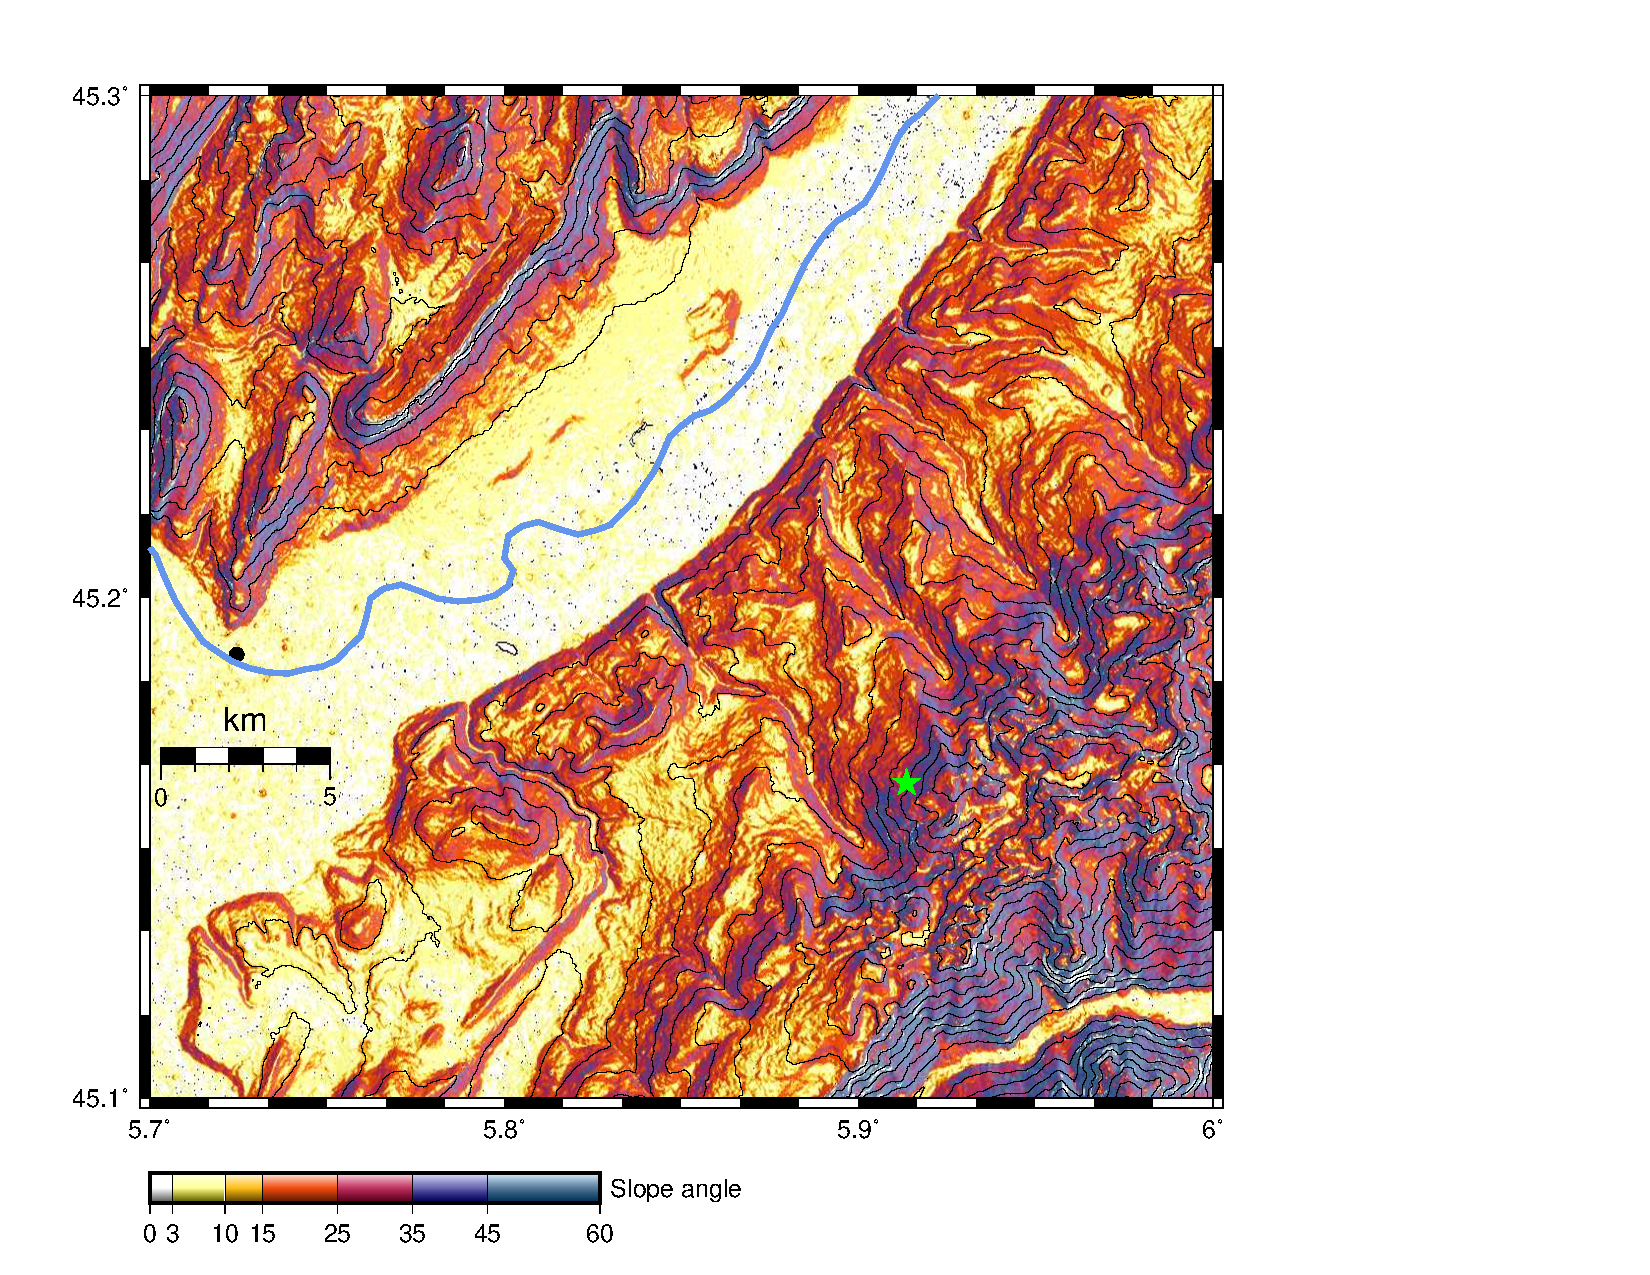
\includegraphics[width=0.8\textwidth]{fig/chapter_1/grenoble_slopes_C100.png}
  \caption{}
  \label{fig:obs_site}
  \end{center}
\end{figure}

The slope in the observational site is around $21\degree$. The meteorological station is going to be located at an altitude of 1770 metres above sea level~\citep{claudine}. All the characterisation of the topography has been done by \cite{alban}.

\subsection{Instrumentation} \label{instrumentation}
The instruments for the next field campaign will be assembled into two masts, which will be located side by side. The mast has been reconfigured to tackle some of the problems and limitations from previous campaigns. We distinguish them by their height, one is 6~m high and the other is 12~m high\footnote{The configuration was altered recently, but couldn't get the most recent schematics. These will certainly change for the presentation.}. 

In figure~\ref{fig:mast_6} we can see the mast that is 6~m high. In it, there are 6 CSAT3 3-D Sonic Anemometers, positioned from 0.4~m to 3.6~m height. These are fixed parallel to the ground. These instruments measure the direction and speed of wind in its three components with a high frequency (around 20~Hz). Currently, Aravind Anandan is doing his research project on the calibration of this instruments and part of his work is calibrating them for this winter mission.

\begin{figure}[!ht]
  \begin{center}
  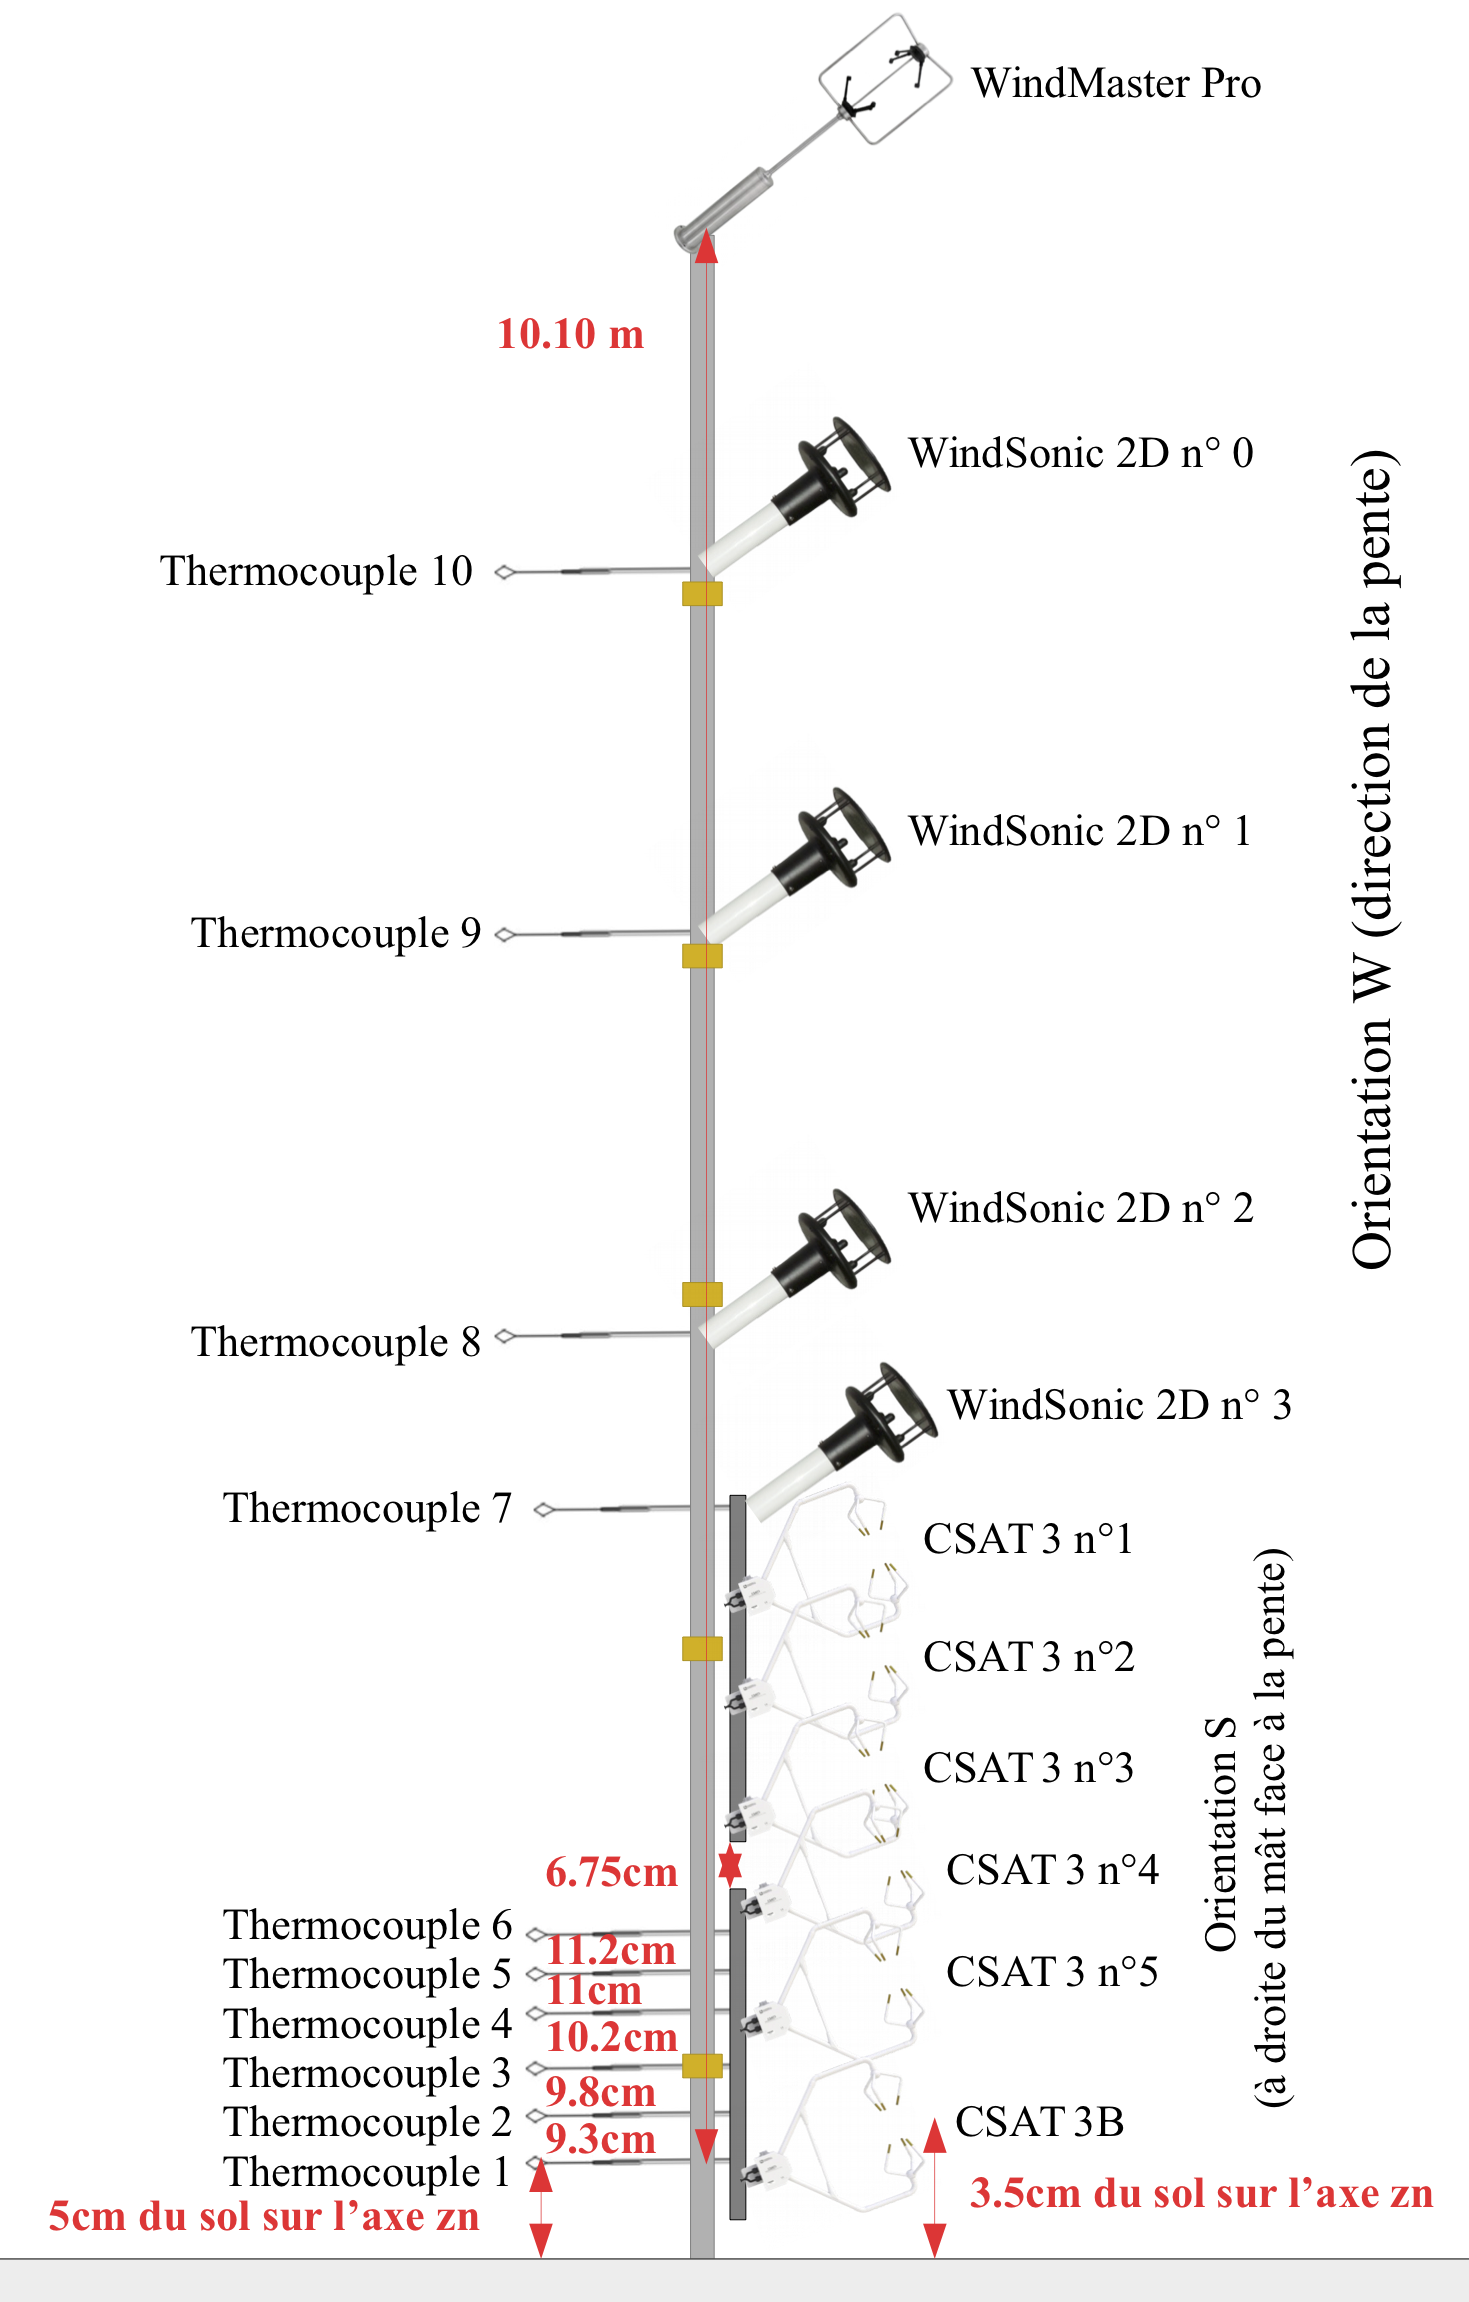
\includegraphics[width=0.7\textwidth]{fig/chapter_1/Montage_J1.png}
  \caption{Placement of the instruments on the 6~m mast. Along the mast, there are six CSAT3 Sonic Anemometers.}
  \label{fig:mast_6}
  \end{center}
\end{figure}

In figure.. we see the mast that is 12~m high. At the top we can see a Windmaster 3D ultrasonic anemometer, that can measure the three components of wind with a frequency up to 20~Hz. Bellow it, we can see three Gill Windmaster anemometers, that are located between 9.5~m and 5.5~m. And at 4.2~m, there is a Vaisala 2D anemometer.  All the anemometers measure the direction and speed of wind with a frequency that depends on the model of the sensor. 

Spread along the mast, there are nine thin film thermocouples, that are used to measure the temperature of air with minimal intrusion. In the middle, there is a radiometer used to measure the radiant flux. Finally, there is an ultrasonic instrument installed in the station (not shown in the figures) to record the height of the snow cover. Snow-covered ground is expected in the measuring site. This is important because the snow decreases the height between the ground and the instruments, which is an important parameter in the calculations.

\section{Timetable}
The timetable~\ref{table:schedule} shows the planning for the activities to do during the next five months. 

\begin{table}[ht!]
%\centering
\begin{center}
\begin{tabular}{|c|c|p{9.5cm}|}
\hline
  & \textbf{Working days} & \textbf{Activity} \\
\hline
January & 1 & Field Work\footnote{\label{note1}The date of the field campaign is not set. It must occur during winter (January and February), when there are anticyclonic conditions.}. Working on theory and foundations of the research.\\
\hline
February & 7 & Field Work$^2$. Analysis of the data, start to analyse 2015 data to get familiar with EddyPro.\\
\hline
March & 4 & Analysis of the data gathered during the field work.\\
\hline
April & 7 & Writing and analysing the data gathered.\\
\hline
May & 12 & Plotting the results and final analysis of the data sets. Working in the final report and oral presentation.\\
\hline
\end{tabular}
\caption{Research project schedule showing the number of working days per month and the tasks to work on.}
\label{table:schedule}
\end{center}
\end{table}

\section{Methodology} \label{sec:methodology}
\subsection{Observational site}

The field campaign occurred in the west face of the Grand Colon mountain (2394~meters) in the Belledonne Massif, 15~km East of Grenoble. A topographic map of the area is shown in figure~\ref{fig:obs_site}, where the measuring site is marked with a green star. The west face of the mountain was selected because it gives direct exposure to solar radiation during the afternoon. This is ideal for katabatic winds to form because the ground cools down after the sun goes down.

\begin{figure}[!ht]
  \begin{center}
  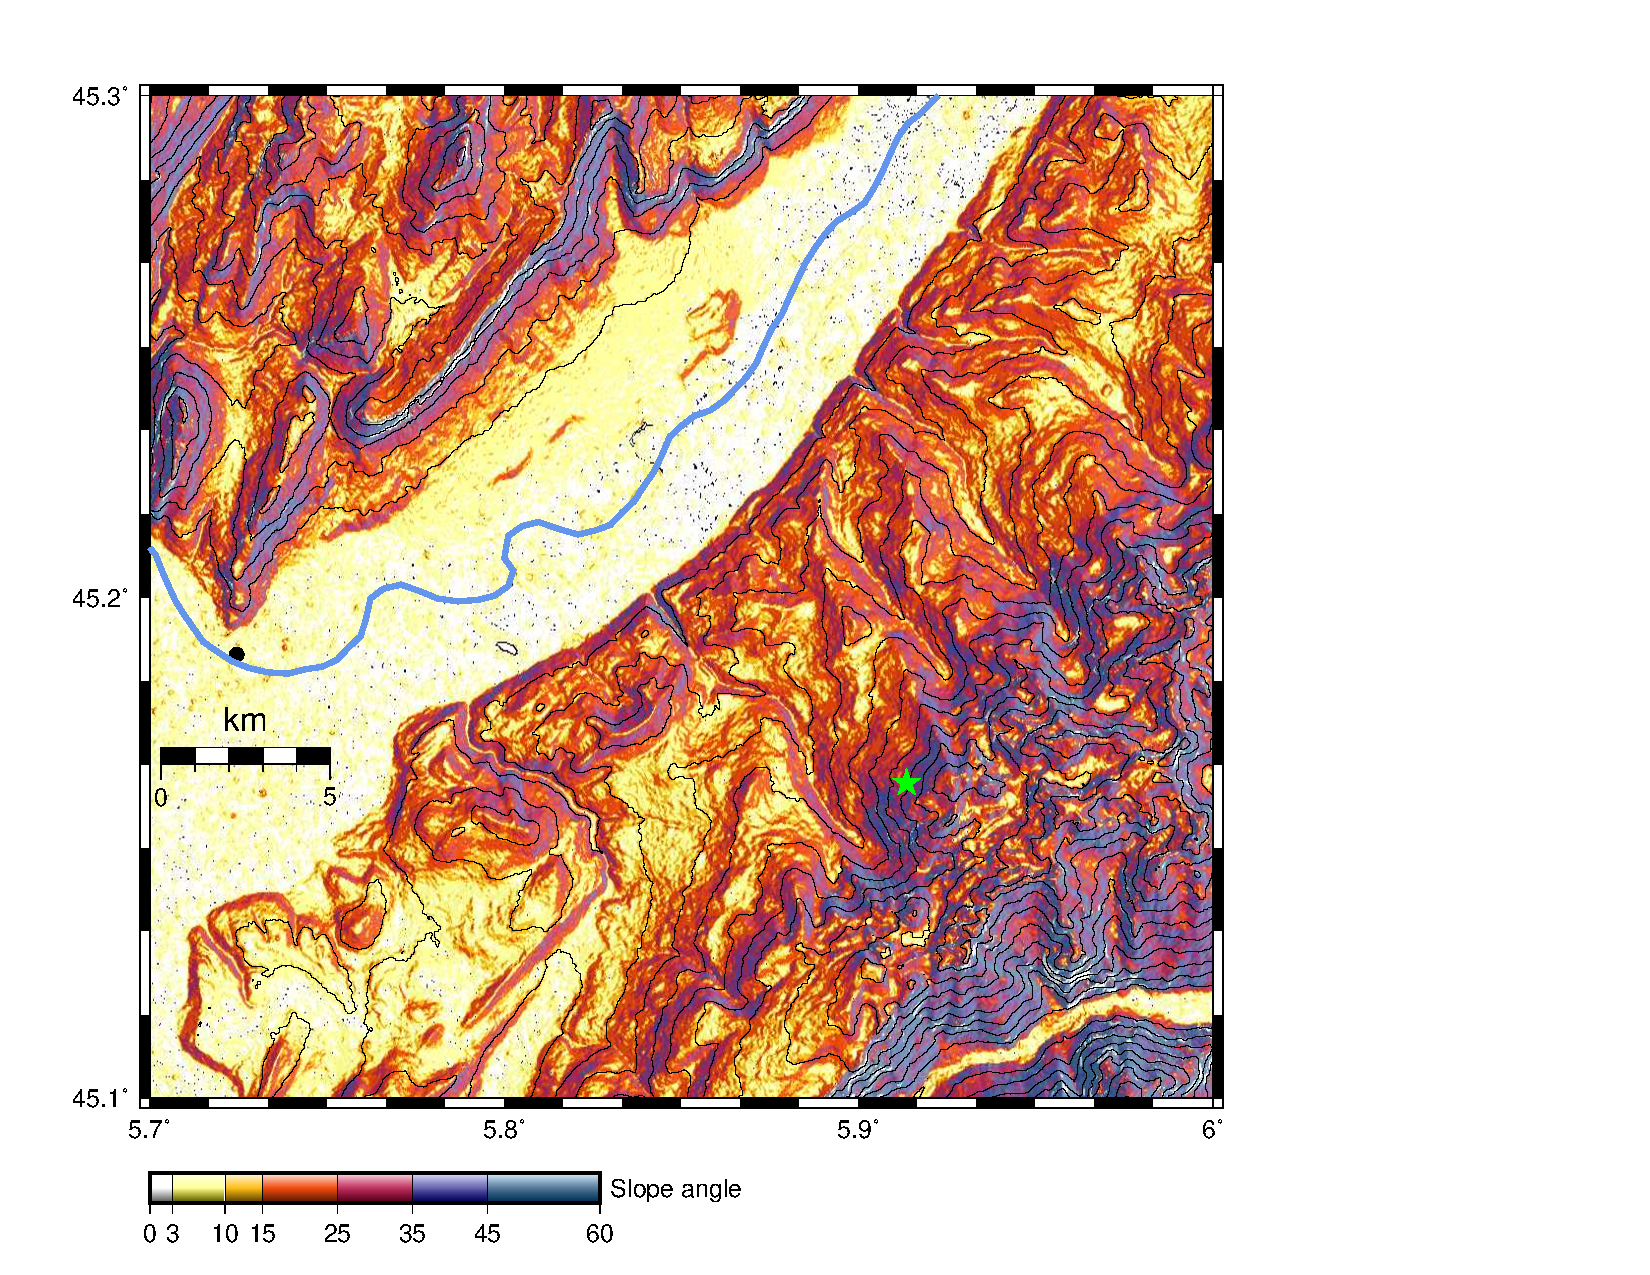
\includegraphics[width=0.8\textwidth]{fig/chapter_1/grenoble_slopes_C100.png}
  \caption{Topographic map showing the slopes of the region. The green star marks the position of the measuring site. The black dot marks the localisation of Grenoble. Data obtained from Shuttle Radar Topography Mission using the GMTSAR processing system~\citep{sandwell2011gmtsar}.}
  \label{fig:obs_site}
  \end{center}
\end{figure}

The meteorological station with the instruments was located at 1770~m height, located in an alpine pasture area (low vegetation and sparse rocks or pebbles) above the forest area and
has a relatively homogeneous slope, which fulfils the essential characteristics for a detailed analysis of the physical process~\citep{blein2016observation}. In particular, the ground was covered by a layer of snow which thickness decreased during the field campaign. The average slope of the site is 30~$\degree$ and it can be seen in the zoomed map in figure~\ref{fig:obs_site_zoom}.

\begin{figure}[!ht]
  \begin{center}
  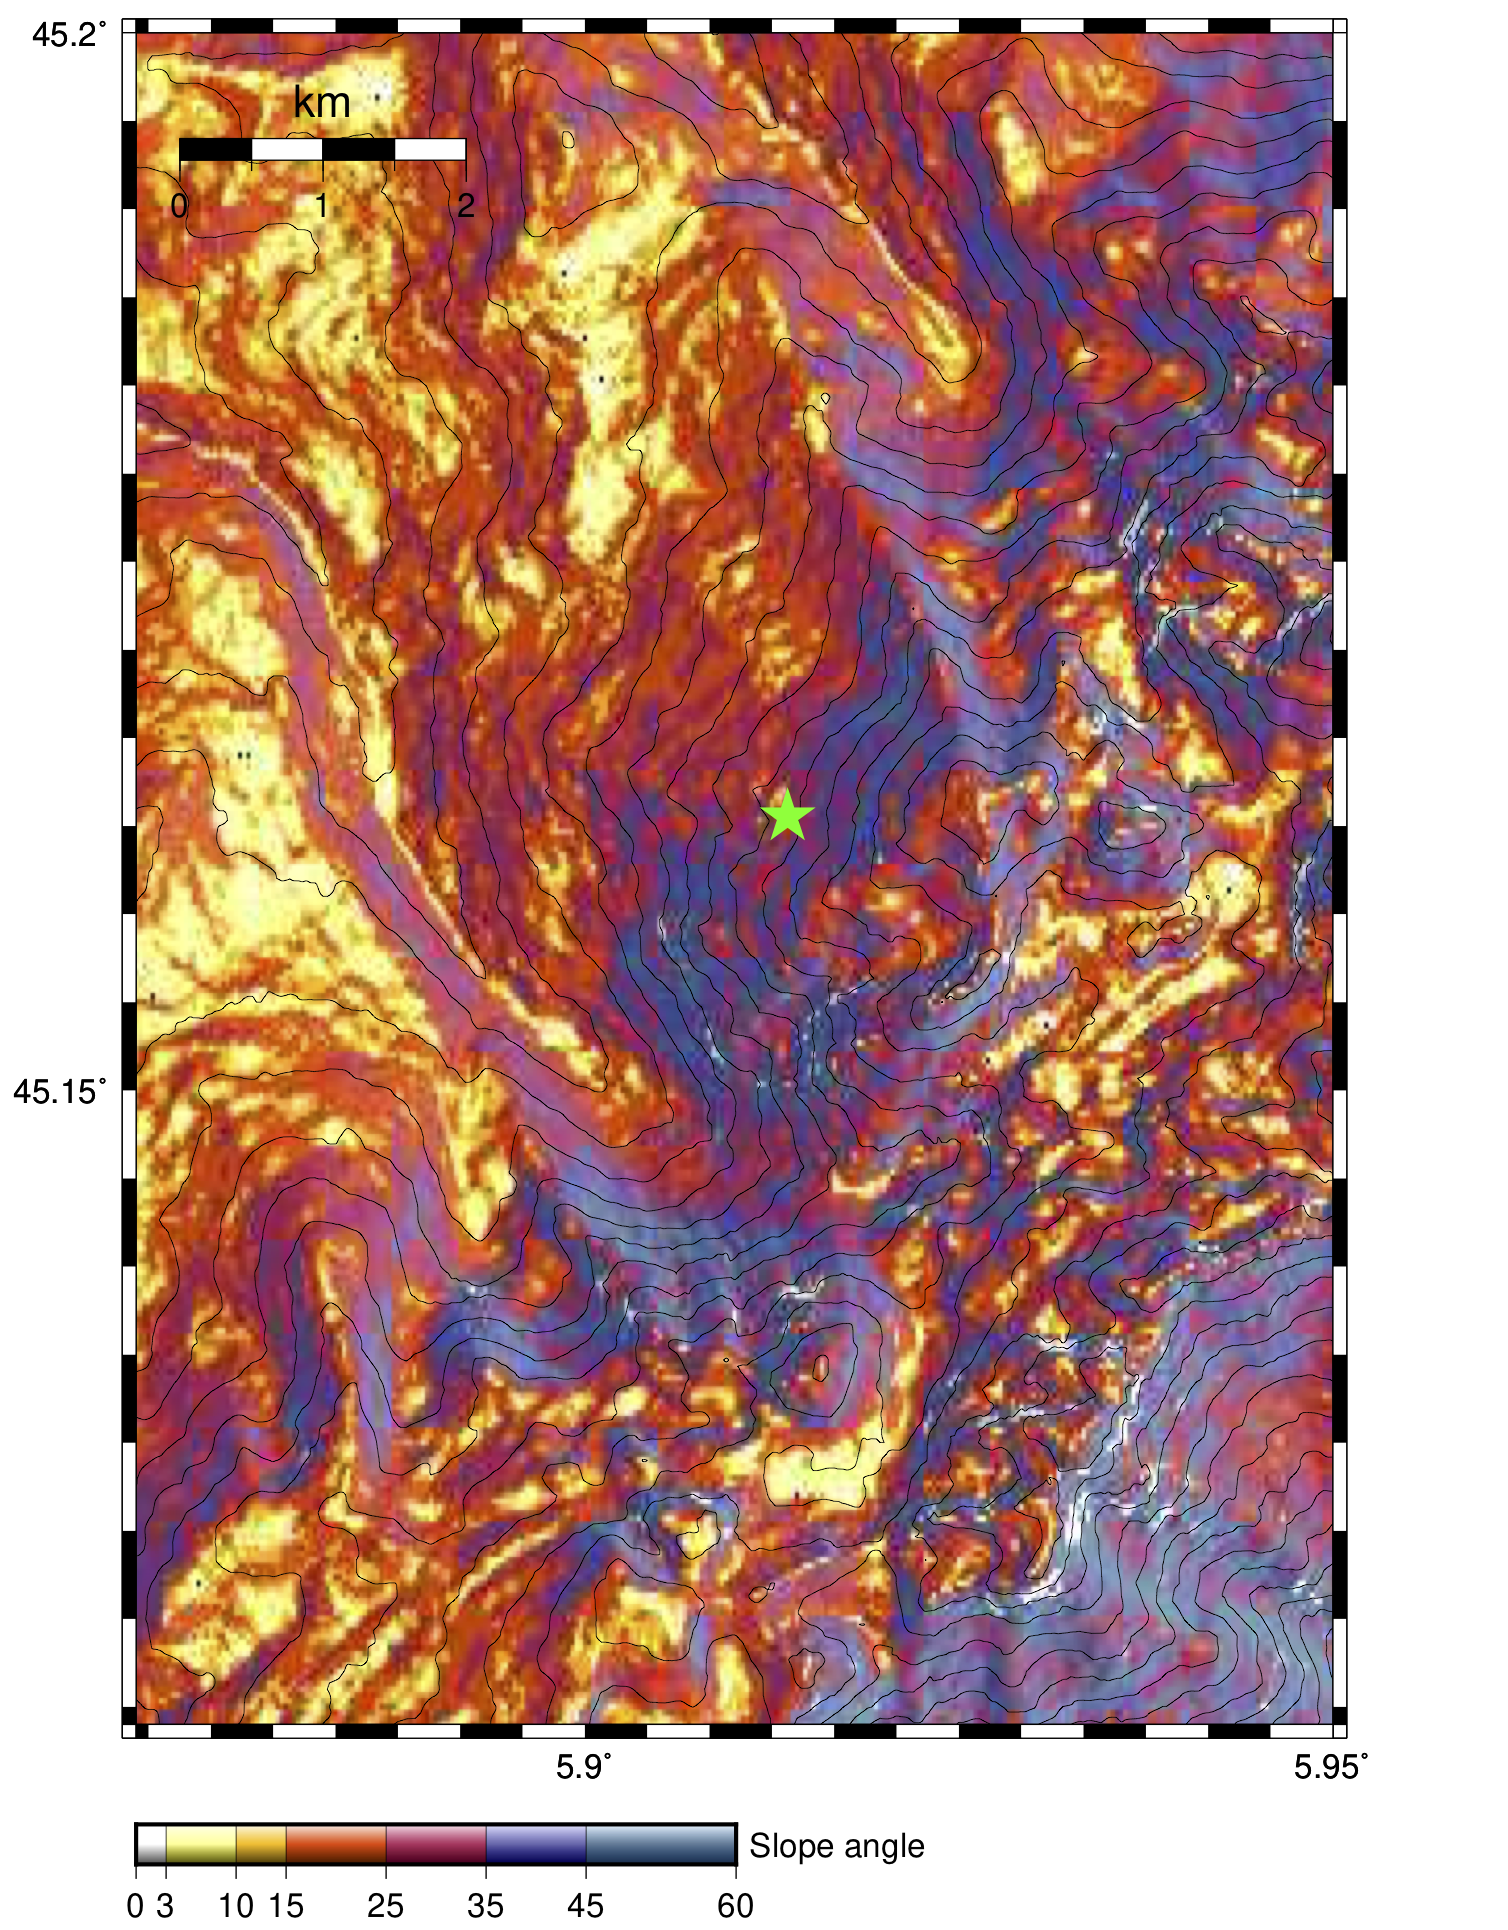
\includegraphics[width=0.5\textwidth]{fig/chapter_1/grenoble_slopes_C100_zoom.png}
  \caption{Zoomed slope map of the area of study. The green star marks the localisation of the instruments.}
  \label{fig:obs_site_zoom}
  \end{center}
\end{figure}

\subsection{Instrumentation} \label{instrumentation}

The instruments placed in the filed where mounted into two masts. The principal mast measured 10.10~m and on it were mounted 11 sonic anemometer and 10 thermocouples (see figure~\ref{fig:mast}). There was a smaller mast with a meteorological station placed a few meters apart from the main mast. It measured temperature, humidity and incident and reflect radiation. In the big mast, there were four types of anemometers with different characteristics and only one type of thermocouple.

The anemometers used were the CSAT3 and CSAT3B~\footnote{The CSAT3B is the most recent version of the CSAT3 but share the same aspect generally.} 3-D sonic anemometers manufactured by Campbells Scientific, which measure three components of the wind with a frequency of 20~Hz. In total there were five CSAT3 and only one CSAT3B. Also, we used four Windsonic 2-D sonic anemometers manufactured by Gill Instruments. This anemometer measures two components of the wind that are aligned to the "plane" of the instrument. At the top of the mast, a Windmater Pro Sonic Anemometer (from Gill Instruments) was placed. As the CSAT3, it measured three components of the wind with a frequency of 20~Hz. In the table~\ref{tab:intruments_anemometers} is possible to see the initial heights at which the anemometers were placed with respect to the ground. 

\begin{table}[!ht]
    \centering
    \begin{tabular}{ | l | c | c | c |}
    \hline
    \textbf{Instrument} & \textbf{Variables measured} &  \textbf{Frequency (Hz)} & \textbf{Height (m)} \\ [0.5ex]  \hline\hline
    CSAT3B & (u,v,w) and Temp. & 20 & 0.035 \\
    \hline
    CSAT3 No.5 & (u,v,w) and Temp. & 20 & 0.36 \\
    \hline
    CSAT3 No.4 & (u,v,w) and Temp. & 20 & 0.67 \\
    \hline
    CSAT3 No.3 & (u,v,w) and Temp. & 20 & 1.16 \\
    \hline
    CSAT3 No.2 & (u,v,w) and Temp. & 20 & 1.57 \\
    \hline
    CSAT3 No.1 & (u,v,w) and Temp. & 20 & 1.98 \\
    \hline
    Windsonic 2D No.3 & (u,v) & 0.003 &  2.7\\
    \hline
    Windsonic 2D No.2 & (u,v) & 0.003 &  3,69\\
    \hline
    Windsonic 2D No.1 & (u,v) & 0.003 &  5.42\\
    \hline
    Windsonic 2D No.0 & (u,v) & 0.003 &  7.02\\
    \hline
    Windmaster Pro & (u,v,w) and Temp. & 20 & 8.97 \\
    \hline
    
    \end{tabular}
    \caption{Caption}
    \label{tab:intruments_anemometers}
\end{table}

An important aspect of the anemometers is its orientation and alignment with respect to the slope. In this case, we aligned all the anemometers in a manner that the horizontal wind components of the instruments were parallel to the slope surface and the vertical wind component perpendicular to the surface (you can see how the instruments are tilted, following the slope of the mountain, in the figure~\ref{}). The orientation of the instruments was different for the CSAT3, the Windsonic 2-D and the Windmaster Pro. The CSAT3 and CSAT3B were oriented towards the south (180~$\degree$ North off-set), in a way that the $v$ component of the wind was facing the slope (eastwards) and the $u$ was facing the right side of the slope (southwards). The Windsonic 2-D was oriented towards the West (270~$\degree$ North off-set) in a manner that the negative $u$ component was facing the slope (it was facing the towards the valley or towards the West). And the Windmaster Pro was facing towards the slope or facing East (90~$\degree$ North off-set).

\begin{figure}[!ht]
  \begin{center}
  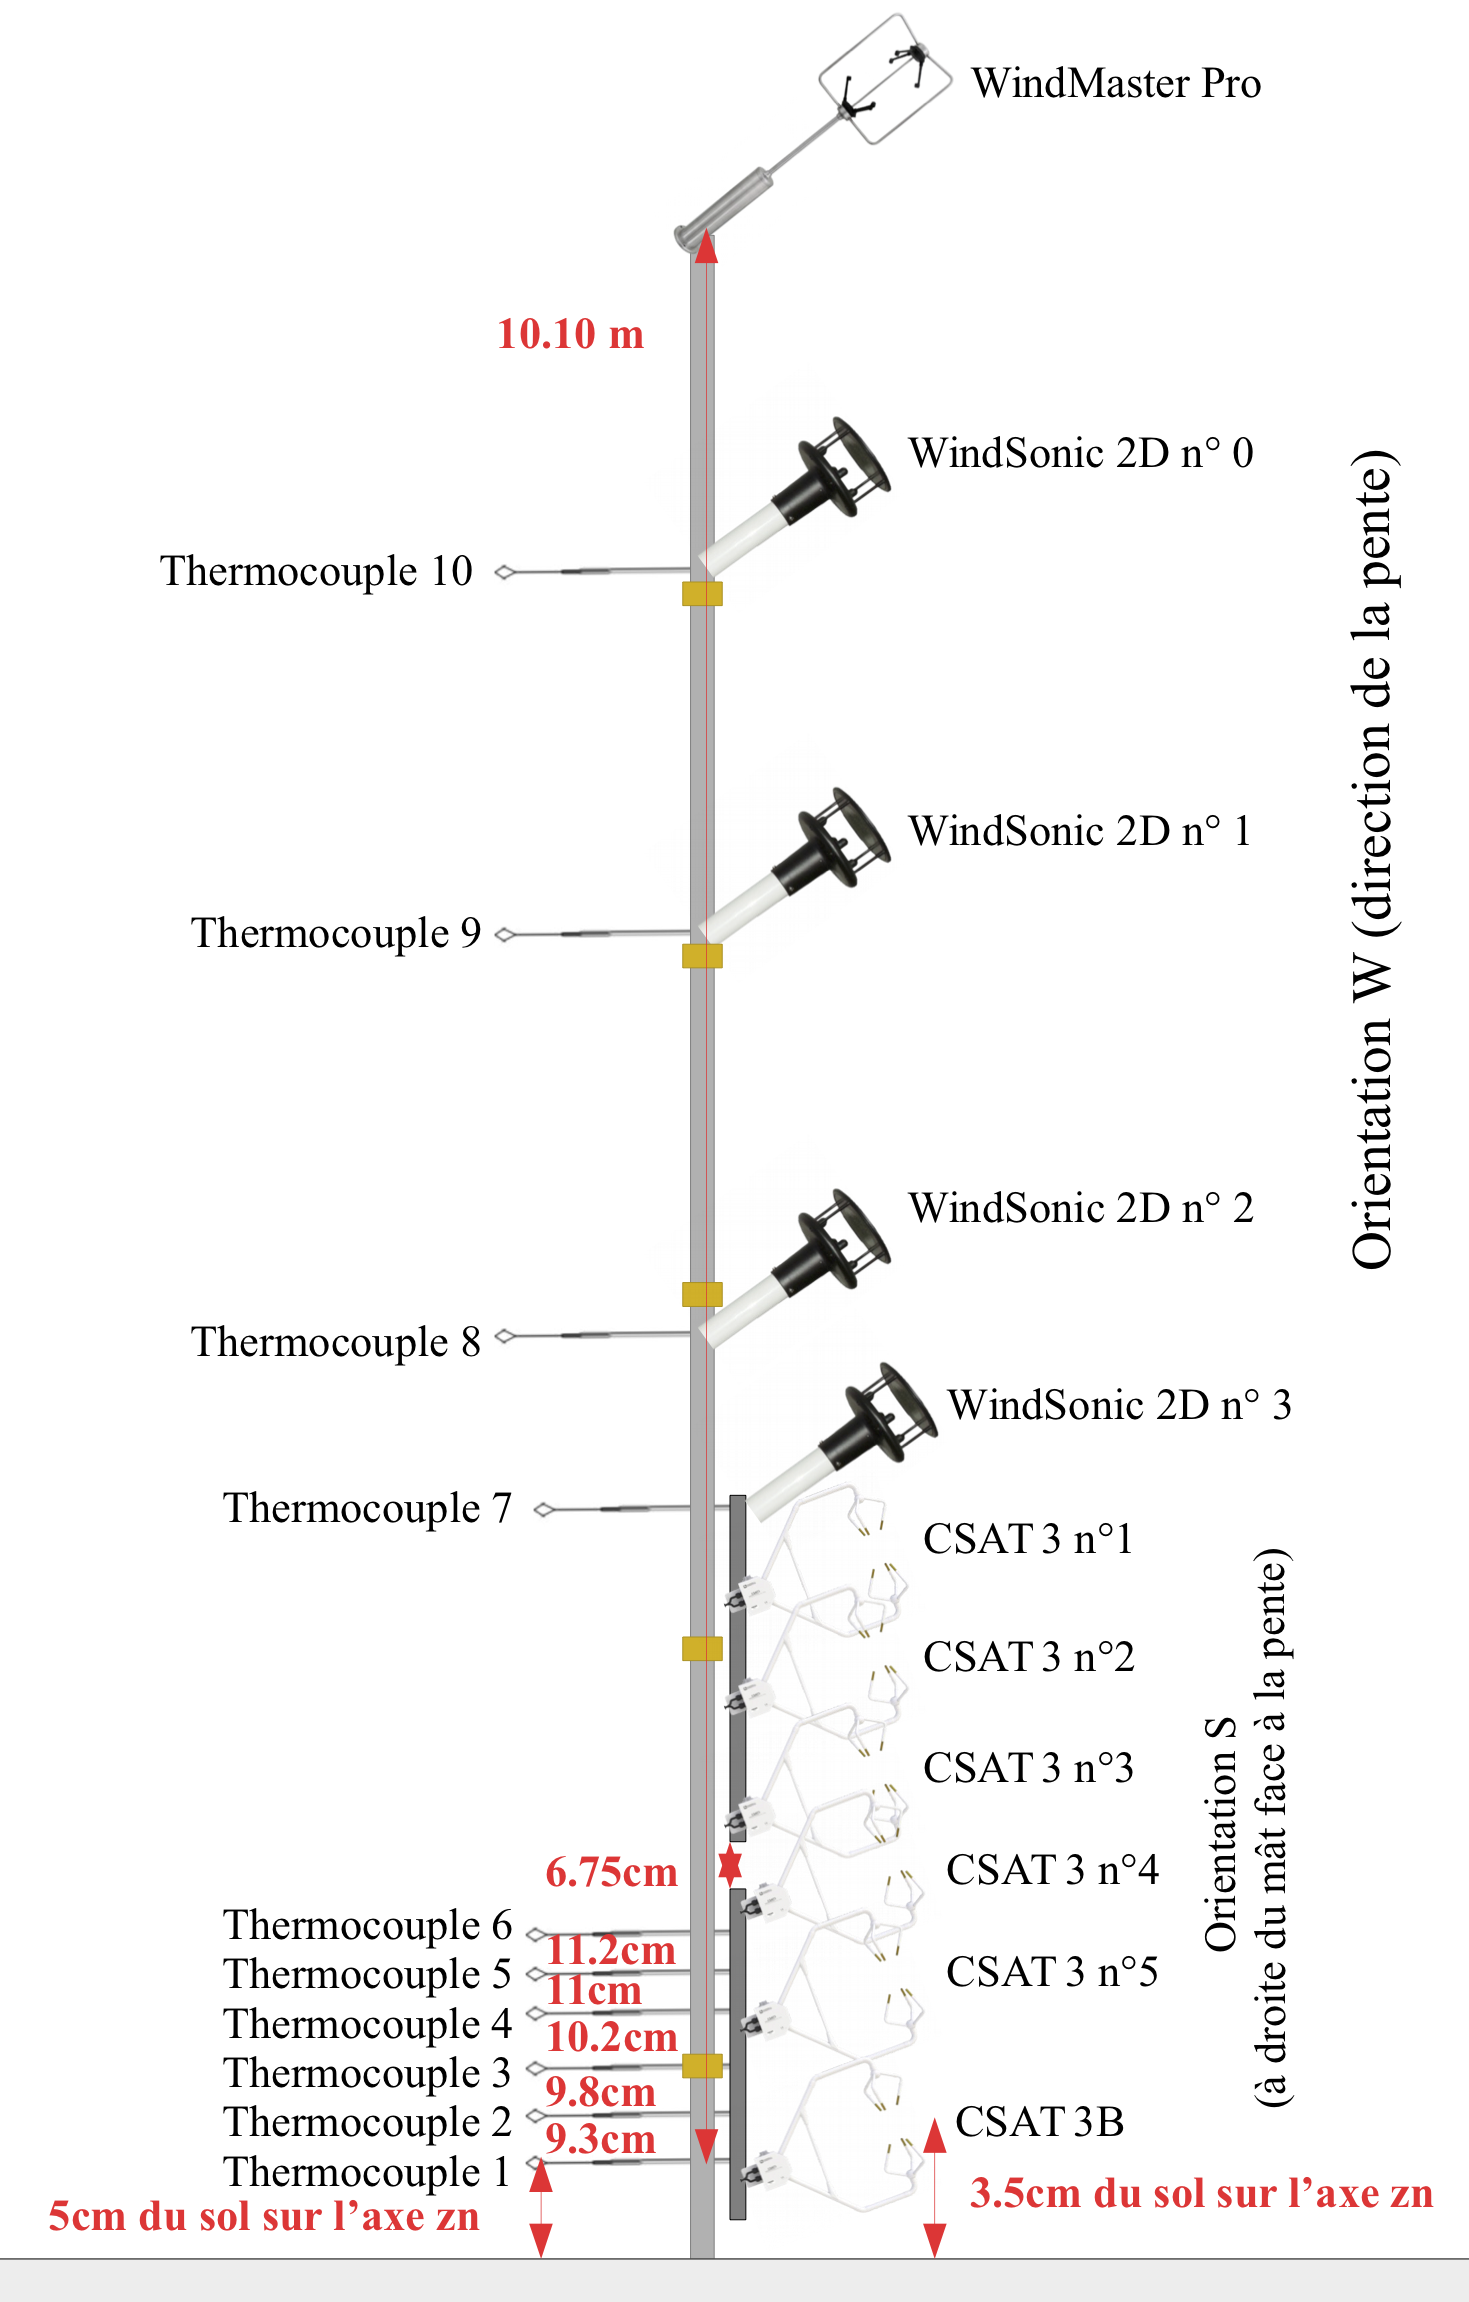
\includegraphics[width=0.7\textwidth]{fig/chapter_1/Montage_J1.png}
  \caption{Placement of the instruments on the 6~m mast. Along the mast, there are six CSAT3 Sonic Anemometers.}
  \label{fig:mast}
  \end{center}
\end{figure}

Spread along the mast, there are ten thin film thermocouples, that were used to measure the air temperature with a minimal intrusion at high frequency (20~Hz). The initial heights of these instruments are shown in table~\ref{tab:intruments_thermocouples} and can be seen in figure~\ref{fig:mast} at the left of the mast, opposite to the anemometers.

\begin{table}[!ht]
    \centering
    \begin{tabular}{ | l | c | c | c |}
    \hline
    \textbf{Instrument} & \textbf{Variables measured} & \textbf{Frequency (Hz)} & \textbf{Height (m)} \\ [0.5ex]  \hline\hline
    Thermocouple No.1 & Temperature & 20 &  0.05\\
    \hline
    Thermocouple No.2 & Temperature & 20 &  0.13\\
    \hline
    Thermocouple No.3 & Temperature & 20 &  0.21\\
    \hline
    Thermocouple No.4 & Temperature & 20 &  0.29\\
    \hline
    Thermocouple No.5 & Temperature & 20 &  0.38\\
    \hline
    Thermocouple No.6 & Temperature & 20 &  0.47\\
    \hline
    Thermocouple No.7 & Temperature & 20 &  2.53\\
    \hline
    Thermocouple No.8 & Temperature & 20 &  3.52\\
    \hline
    Thermocouple No.9 & Temperature & 20 &  5.26\\
    \hline
    Thermocouple No.10 & Temperature & 20 & 6.84 \\
    \hline
    
    \end{tabular}
    \caption{Caption}
    \label{tab:intruments_thermocouples}
\end{table}

In the middle, there is a radiometer used to measure the radiant flux. Finally, there is an ultrasonic instrument installed in the station to record the height of the snow cover (snow-covered ground was expected in the measuring site). This is important because the snow decreases the height between the ground and the instruments, which is an important parameter in the calculations.

\subsection{Field campaign}

The field campaign could only take place during certain weather conditions and during winter. For this reason, we couldn't establish a certain date for it. First of all, winter is the season when the occurrence of katabatic winds event is greater because of the cold temperatures in the mountains. Also, the other important factor, as mentioned in section~\ref{sec:katabatic_winds}, is that the presence of mesoscale wind systems can overshadow or inhibit the formation of katabatic winds. For this reason, an ideal weather condition for measuring katabatic winds is during anticyclonic events, in which mesoscale wind systems are weak, the skies are clear and the air is cooler.

During the month of February, between the 10th and the 28th,  Grenoble had anticyclonic weather conditions that were brought by three high-pressure systems that passed over the region during this period of time, these were named: Dorit, Erika and Frauke. This meteorological window allowed us to carry out the field campaign. In total, the instruments took measurements for 17 days.

\subsection{Data processing}

In total around 11.5~GB were obtained during the campaign, only taking into account the anemometers, the thermocouples and the meteorological station. The processing of the data depended on the instrument and its frequency of operation. 

\subsubsection{EddyPro data processing}

For the CSAT3 anemometers and the Windmaster Pro we used EddyPro, which is a software that uses the eddy covariance method to compute atmospheric fluxes of certain trace gases, heat flux and energy~\citep{burba2013eddy}. EddyPro computes the averages of each of the components of the wind and the temperature for a certain period of time which we choose. After this, it computes the fluctuations of the variables and computes the covariance between them. There are multiple choices for software that can do this but EddyPro integrates different functions and methods that improve the quality of the output. 

The raw data of the sonic anemometers is in ASCII format, which EddyPro con read only pointing out what are the columns corresponding to each variable and each instrument. For this also we have to specify the height of the instruments with respect to the ground, the orientation of the instruments with respect to the north, the type of average to compute and the period for computing the average. 

Due to the number of days the instruments were operating and the high frequency of acquisition, it was convenient to use a relatively large period for averaging to try to identify the days when there were good conditions for katabatic winds to form. For this reason, we processed the data doing 30 minutes averages for both the CSAT3 anemometers and the Windmaster Pro. This type of average works as a low-pass filter for the raw high-frequency signal, where all the turbulent fluctuations of the variables are lost. For this reason, is only convenient to use this 30~minutes averaged data to identify potential good periods with the required conditions and not to analyse the turbulent characteristics of the flow

After identifying three potentially good nights for katabatic winds episodes, we went back to EddyPro and processed the data using a 5~minutes average period, which works better to analyse the turbulent characteristics of the flow and the respective fluxes. 

\subsubsection{Thermocouples and WindSonic anemometers}







\section{Results}
The CSATS didn't operated for the full campaign. They were functioning from the 12th to the 17th and from the 19th to the 28th of February, so they were inactive during two days. In the case of the Windmaster Pro, it was operating from the 19th to the 28th of February. 

\section{Conclusion}
The calibration done between the different type instruments showed that there was consistency between the temperature of the Thermocouples and the CSAT3's, measured at similar heights. Although, there was a significant horizontal separation between the CSAT3-B and the Thermocouple No.1 and between the CSAT3 No.4 and the Thermocouple No.4, the measurements where similar, as the high correlation value pointed out. This gave us the confidence of using the measurements of the Thermocouples to characterise the vertical profiles, with the advantage that there were more Thermocouples installed on the mast that CSAT3's to measure the temperature.

Doing the same calibration between the wind speed measured with the lowest Windsonic 2-D and the highest CSAT3, we found that the correlation was of 0.94, which shows that the wind speed of both instruments had the approximate same magnitude, even though there was a vertical separation of 0.7m between them. This is important at the moment of plotting the mean vertical wind profiles because there must be coherence in the measurements done with a different type of instruments for the profile to make sense. 

From the whole campaign, we were able to identify two nights with katabatic winds. As shown by the vertical profiles, the maximum in the mean wind speed was located between 0.5~m and 0.75~m. We expected to find this maximum at a higher level, to have two CSAT3's that could measure the wind below the maximum and two CSAT3's above the maximum, but instead of this, only one anemometer measured the wind below the maximum. 

During the night of the 23rd to the 24th, the momentum fluxes profiles showed a negative flux for the levels below the wind maximum and a positive flux above the maximum, with the exception of some rogue profiles that were negative at all levels or were negative above the wind maximum. Regarding the sensible heat flux, all the profiles were negative because of the stable environment, but there where some variations when the profiles should remain constant. For the TKE, the profiles showed a small value of TKE close to the surface, and an increase of TKE as the height increased, which correspond to what was expected. 

Globally, the campaign was a success because of the 17 days of anticyclonic conditions, which allowed to take sufficient measurements of katabatic winds structure, with better spacial resolution due to the improvements implemented based on previous campaigns. Despite that this work focused only on two nights, there are still many other nights to analyse and a lot of work ahead to do.

\clearpage
%\medskip
%\nocite{*}
\bibliographystyle{apalike}
\bibliography{biblio}
%\printbibliography

\end{document}
